\documentclass[10pt]{article}

\pagestyle{empty}

\setlength{\textheight}{250mm}
\setlength{\textwidth}{180mm}
\setlength{\oddsidemargin}{-8mm}
\setlength{\topmargin}{-1.5cm}

\usepackage{amsmath}
\usepackage{amsthm}
\usepackage{psfrag}
\usepackage{graphicx}
\usepackage{bm}
\usepackage{mathrsfs}
\usepackage{icomma} % pacchetto per limitare lo spazio standard posto dopo la virgola in caso che la virgola sia tra cifre
\usepackage{amsfonts} % amplia i caratteri matematici disponibili
\usepackage{amssymb}
%\usepackage{wrapfig}
\usepackage{empheq}

\usepackage{epstopdf}
\usepackage[utf8x]{inputenc}
\usepackage{ifthen}

\usepackage[italian]{babel}
%\usepackage[latin1]{inputenc}

\usepackage{pgfplots}
\pgfplotsset{compat=1.9}

%\input{def}

%\newcommand{\kg}{\textrm{kg}}
%\newcommand{\K}{\textrm{K}}
%\newcommand{\m} {\textrm{m}}
%\newcommand{\dm}{\textrm{dm}}
%\newcommand{\cm}{\textrm{cm}}
%\newcommand{\mm}{\textrm{mm}}
%\newcommand{\s} {\textrm{s}}
%\newcommand{\N} {\textrm{N}}
%\renewcommand{\Pa}{\textrm{Pa}}

\def \flagSect{0} % 1    : numerazione
		  % else : niente
%\newcommand{\taitol}[1]  % stile titolo
%{
%%{\textit{#1}}
%{#1}
%}
\def \soluzione{Soluzione}
\def \partePrima{Concetti. }
\def \parteSeconda{Svolgimento. }
%\def \parteTerza{}
\newcommand{\sol}{\subsubsection*{\soluzione}}
\newcommand{\partone}{\ \ \ \ \ \textbf{\partePrima}}
\newcommand{\parttwo}{\vspace{0.2cm}\textbf{\parteSeconda}}

\ifnum\flagSect=1
\newtheorem{esercizio}{Esercizio}%[section]
\else
\newtheorem*{esercizio}{Esercizio}
\fi

\newtheorem*{teorema}{Teorema}
\newtheorem*{lemma}{Lemma}

% ###########################################################
%\def \flagSect{0} % 1    : numerazione
		  % else : niente
%\newcommand{\taitol}[1]  % stile titolo
%{
%%{\textit{#1}}
%{#1}
%}
\def \soluzione{Soluzione}
\def \partePrima{Concetti. }
\def \parteSeconda{Svolgimento. }
%\def \parteTerza{}
\newcommand{\sol}{\subsubsection*{\soluzione}}
\newcommand{\partone}{\ \ \ \ \ \textbf{\partePrima}}
\newcommand{\parttwo}{\vspace{0.2cm}\textbf{\parteSeconda}}

\ifnum\flagSect=1
\newtheorem{esercizio}{Esercizio}%[section]
\else
\newtheorem*{esercizio}{Esercizio}
\fi

\newtheorem*{teorema}{Teorema}
\newtheorem*{lemma}{Lemma}

% ###########################################################
%\def \flagSect{0} % 1    : numerazione
		  % else : niente
%\newcommand{\taitol}[1]  % stile titolo
%{
%%{\textit{#1}}
%{#1}
%}
\def \soluzione{Soluzione}
\def \partePrima{Concetti. }
\def \parteSeconda{Svolgimento. }
%\def \parteTerza{}
\newcommand{\sol}{\subsubsection*{\soluzione}}
\newcommand{\partone}{\ \ \ \ \ \textbf{\partePrima}}
\newcommand{\parttwo}{\vspace{0.2cm}\textbf{\parteSeconda}}

\ifnum\flagSect=1
\newtheorem{esercizio}{Esercizio}%[section]
\else
\newtheorem*{esercizio}{Esercizio}
\fi

\newtheorem*{teorema}{Teorema}
\newtheorem*{lemma}{Lemma}

% ###########################################################
%\input{logicNumb}
%\newcommand{\sectionIf}[2]
%{
%   \ifthenelse{\equal{#1}{1}}
%              {\subsection{#2}}{\subsection*{#2}}
%}
% ###########################################################

%\newcommand{\sectionIf}[2]
%{
%   \ifthenelse{\equal{#1}{1}}
%              {\subsection{#2}}{\subsection*{#2}}
%}
% ###########################################################

%\newcommand{\sectionIf}[2]
%{
%   \ifthenelse{\equal{#1}{1}}
%              {\subsection{#2}}{\subsection*{#2}}
%}
% ###########################################################

\begin{document}

\begin{center}
\textbf{Esercizi per il corso di Fluidodinamica} 
\medskip
\end{center}



%%%%%%%%%%%%%%%%%%%%%%%%%%%%%%%%%%%%%%%%%%%%%%%%%%%%%%%%%%%%%%%%%%

%%%%%%%%%%%%%%%%%%%%%%%%%%%%%%%%%%%%%%%%%%%%%%%%%%%%%%%%%%%%%%%%%%

%%%%%%%%%%%%%%%%%%%%%%%%%%%%%%%%%%%%%%%%%%%%%%%%%%%%%%%%%%%%%%%%%%


\subsection{Condizione necessaria di incipiente separazione}
Un punto di incipiente separazione viene identificato dall'anullarsi
 della derivata in direzione perpendicolare a parete della componente
 di velocità parallela ad essa, con derivata seconda positiva.
Si consideri il problema bidimensionale su una superficie piana: viene
 scelto di usare un sistema di riferimento cartesiano con l'asse $x$
 parallelo alla parete e diretto nel verso della corrente asintotica
 $\bm{U} = U \bm{x}$, l'asse $y$ uscente dalla parete.
La componente $x$ dell'equazione della quantità di moto è
 \begin{equation}
  u \dfrac{\partial u}{\partial x} +
  v \dfrac{\partial u}{\partial y} -
  \dfrac{1}{Re}\left[ \dfrac{\partial^2 u}{\partial x^2} +
                      \dfrac{\partial^2 u}{\partial y^2} \right] +
  \dfrac{\partial P}{\partial x} = 0
 \end{equation}
A parete i termini non lineari sono nulli poichè la velocità è nulla per
 la condizione di adesione. La derivata seconda in direzione $x$ è nulla
 poichè a parete la velocità è sempre zero per ogni valore della coordinata 
 $x$. Rimane quindi
 \begin{equation}
  \dfrac{\partial P}{\partial x} =
    \dfrac{1}{Re}\dfrac{\partial^2 u}{\partial y^2} > 0
 \end{equation}
 


\noindent
\begin{tabular}{c}
\begin{minipage}[b]{0.95\textwidth}
\begin{exerciseS}[Separazione su parete piana]
Si assuma che il profilo di velocit\`{a} $u(x,y)$ dello strato limite sulla superficie di un corpo
sia approssimabile con la seguente legge
$$
 u = \frac{(1-x)y}{1+y} + \frac{xy^2}{1+y^2},
$$
dove $u$ \`{e} la velocit\`{a} adimensionalizzata rispetto alla velocit\`{a} esterna, $x$ \`{e} la 
coordinata adimensionale di parete localmente rettilinea e $y$ la coordinata adimensionale in direzione
normale alla parete stessa. Determinare la coordinata $x_s$ del punto di separazione dello strato limite
in questione.
\end{exerciseS}
\end{minipage}
\end{tabular}


\sol

\partone
 Separazione.

\parttwo


\begin{equation}
\begin{aligned}
  \frac{\partial u}{\partial y} & = \frac{\partial}{\partial y} \displaystyle \left[
  \frac{(1-x)y}{1+y} + \frac{xy^2}{1+y^2} \right] = \\
  & = (1-x)\frac{1}{(1+y)^2} + x \frac{2y}{(1+y^2)^2}
\end{aligned}
\end{equation}

Quando si impone la condizione di separazione $\frac{\partial u}{\partial y}\big|_{y=0} = 0$, si ottiene $x_s = 1$.

\begin{figure}[h!]
  \centering
   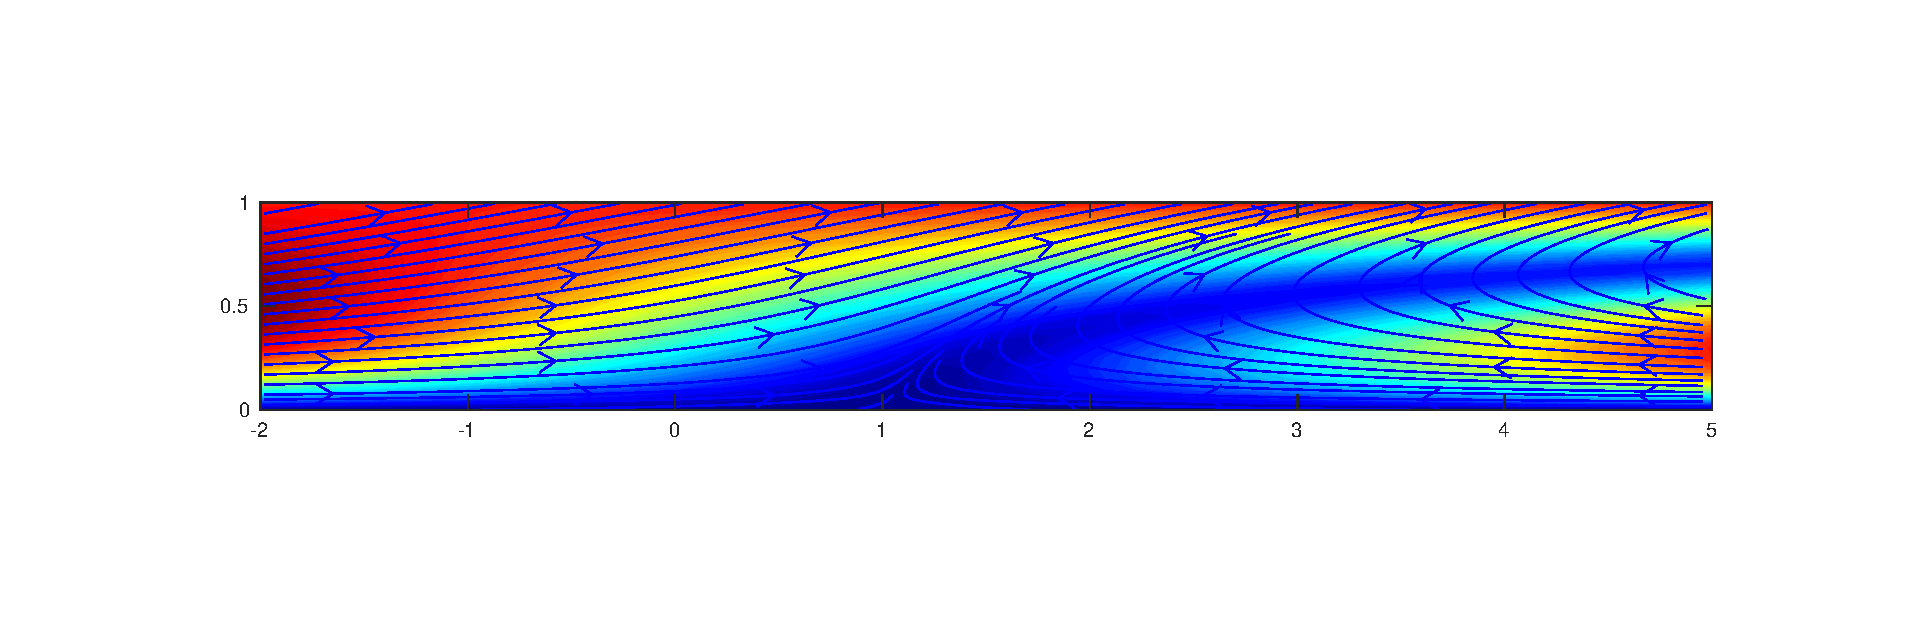
\includegraphics[width=0.90\textwidth,trim = {10mm 30mm 10mm 20mm}, clip]{./fig/Ese75contour.eps}
   \caption{Linee di corrente e modulo della velocità.}
\end{figure}

\begin{figure}[h!]
\centering
   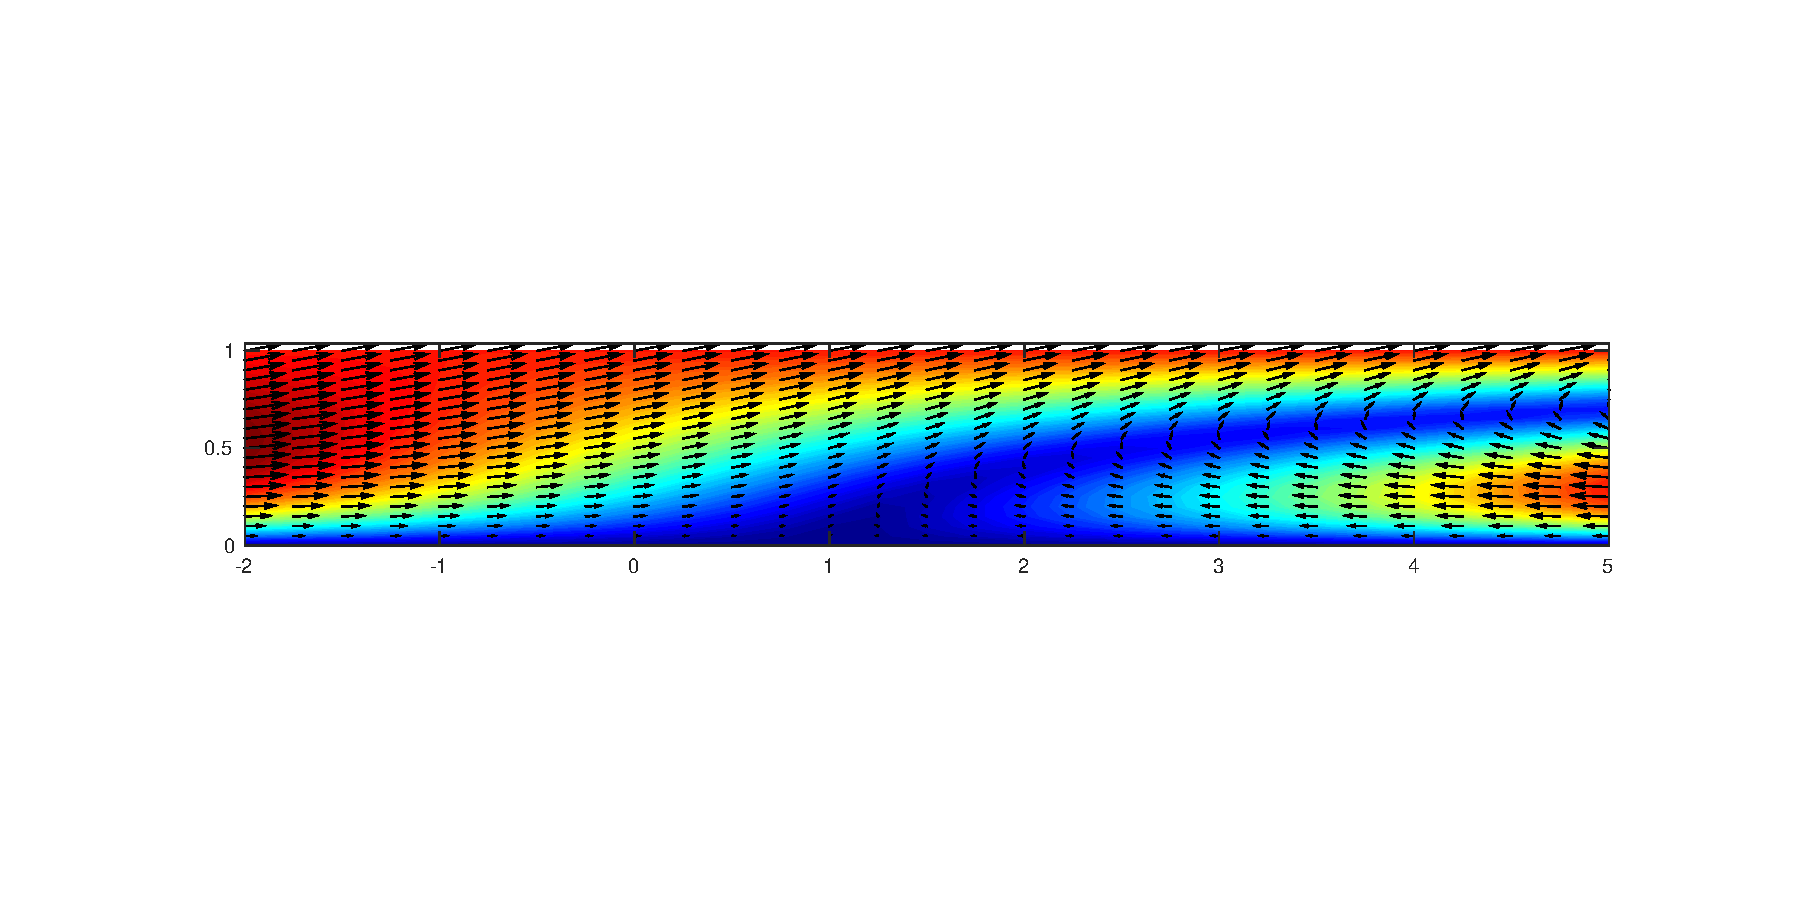
\includegraphics[width=0.90\textwidth,trim = {10mm 50mm 10mm 40mm}, clip]{./fig/Ese75quiver.eps}
   \caption{Campo di velocità e modulo della velocità.}
\end{figure}

\begin{figure}[h!]
\centering
   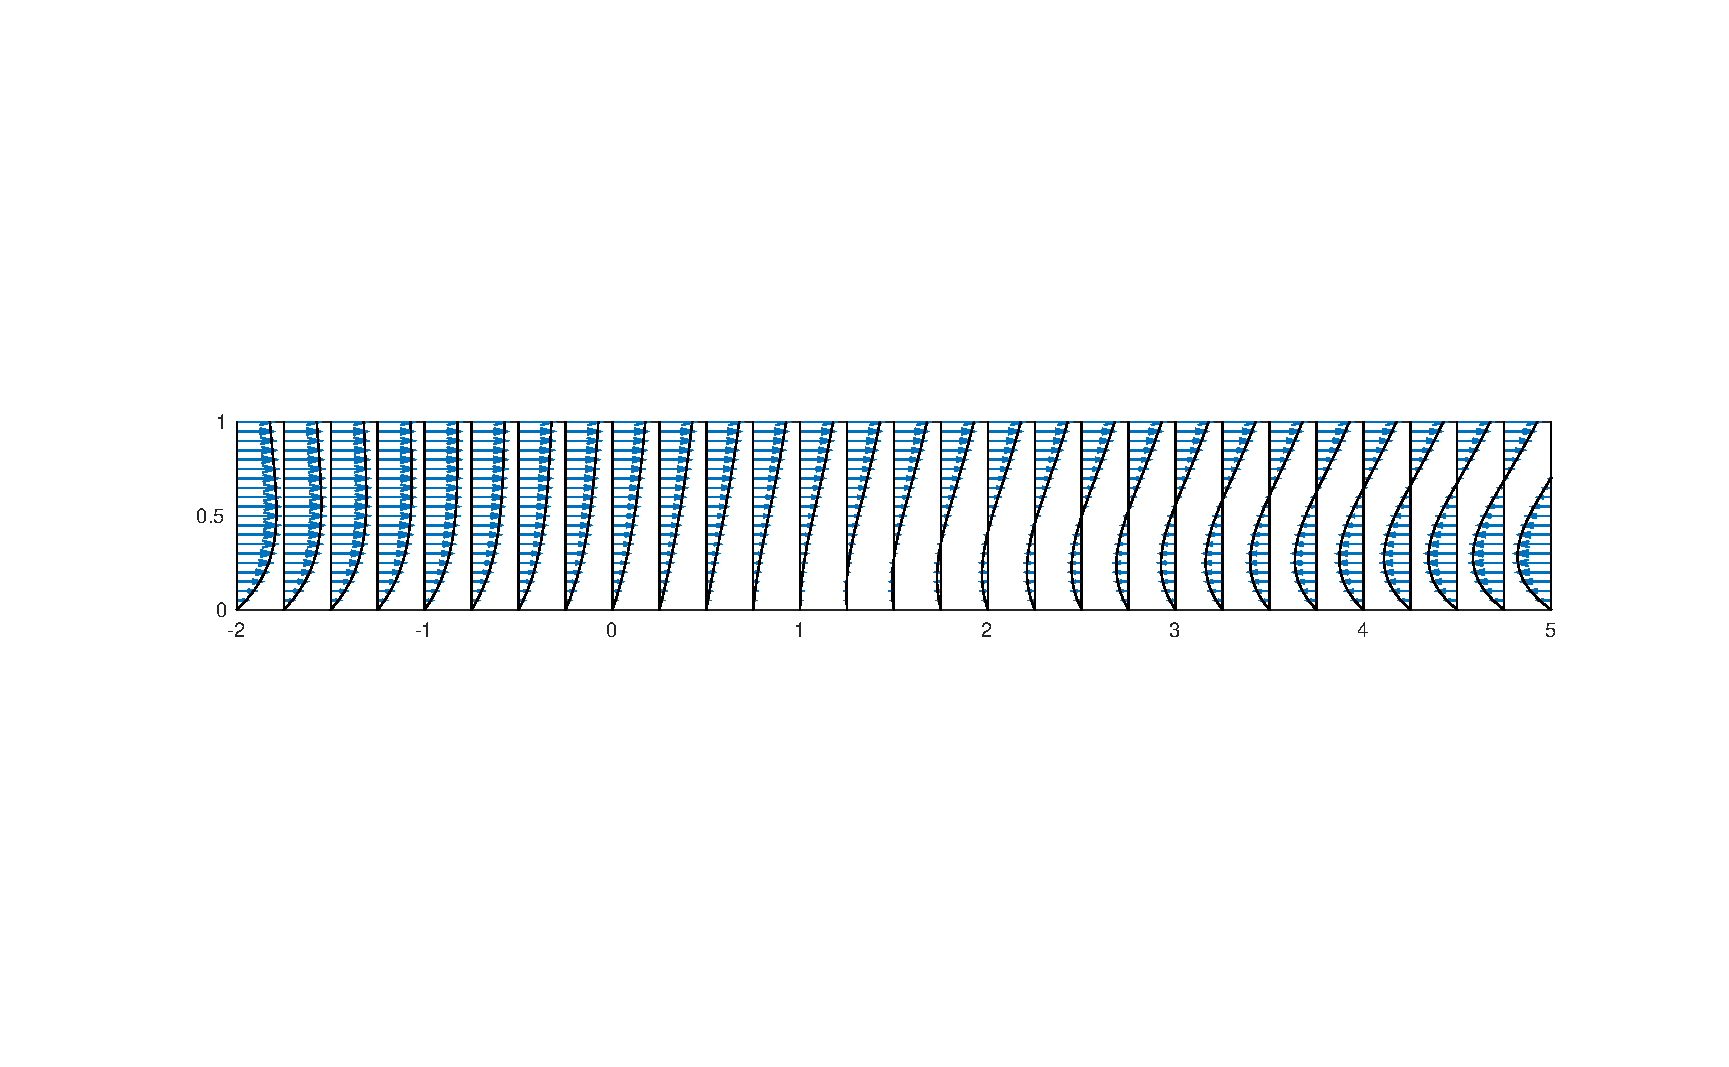
\includegraphics[width=0.90\textwidth,trim = {10mm 60mm 10mm 60mm}, clip]{./fig/Ese75u.eps}
   \caption{Andamento della componente orizzontale $u(y)$ in diverse stazioni x.}
\end{figure}

Se si ipotizza che il moto del fluido sia governato dalle equazioni di 
 Navier-Stokes per fluido incomprimibile (così facendo, si abbandonano
 le ipotesi di non viscosità del fluido e irrotazionalità della corrente, 
 proprie dell'Aerodinamica; in realtà questo è già stato fatto nel testo
 del problema, imponendo un profilo di velocità che soddisfa la condizione
 di adesione a parete...) è possibile ricostruire il campo di velocità e di 
 pressione. Utilizzando il vincolo di incomprimibilità e le condizioni
 al contorno a parete ($y=0$), si può calcolare la componente di velocità
 $v(x,y)$ perpendicolare alla parete
 \begin{equation}
  v(x,y) = - ln | 1 + y | + atan \ y
 \end{equation}
 Utilizzando le equazioni stazionarie di Navier-Stokes è possibile 
 determinare il campo di pressione $P(x,y)$. La pressione (a meno di 
 costanti di integrazione) e la derivata in direzione $x$ valutate
 a parete valgono
 \begin{equation}
 \begin{cases}
  P(x,0) & = \dfrac{1}{Re} ( 2 x^2 - 2 x ) \\
  \dfrac{\partial P}{\partial x}(x,0) & = \dfrac{1}{Re} ( 4 x - 2 )
 \end{cases}
 \end{equation}
 Si noti che nel punto di separazione $x_s=1$, la derivata $\partial P/
 \partial x (x_s,0) = 2 / Re$ è positiva (come era logico attendersi, per la
 condizione necessaria di incipiente separazione).

 
 

%\begin{figure}[h!]
%\centering
%   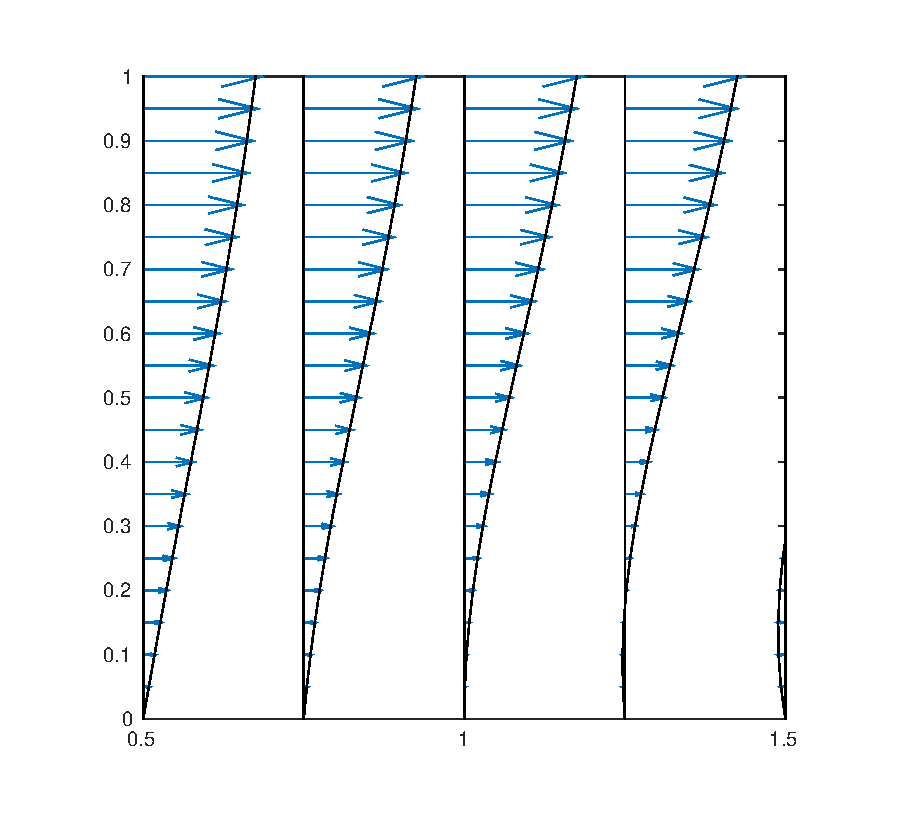
\includegraphics[width=0.90\textwidth]{./fig/Ese75uSep.eps}
%   \caption{Ingrandimento sul punto di separazione.}
%\end{figure}



%%%%%%%%%%%%%%%%%%%%%%%%%%%%%%%%%%%%%%%%%%%%%%%%%%%%%%%%%%%%%%%%%%

%%%%%%%%%%%%%%%%%%%%%%%%%%%%%%%%%%%%%%%%%%%%%%%%%%%%%%%%%%%%%%%%%%
%%%%%%%%%%%%%%%%%%%%%%%%%%%%%%%%%%%%%%%%%%%%%%%%%%%%%%%%%%%%%%%%%%

\end{document}
